\section{matplotlib}

\subsection{\texttt{figure}オブジェクトと\texttt{axes}オブジェクトの作成}
一つ一つのグラフの本体は,matplotlibでは\texttt{<axes>}として表され,\texttt{<axes>}は,\texttt{<figure>}の中で管理される.イメージとしては、\texttt{<figure>}は白のキャンバスであり,そこにグラフの素である\texttt{<axes>}を置いていく.空の\texttt{<axes>}は,デフォルトの軸だけがセットされている.

\begin{gram} 
\begin{itemize}
\item \texttt{plt.figure()}: 空の\texttt{<figure>}を作成する.
\item \texttt{<figure>.add\_subplot(a,b,c)}: \texttt{<figure>}を\texttt{a}行\texttt{b}列に分割した上で,\texttt{c}番目の部分に空の\texttt{<axes>}を作成する.
\item \texttt{<figure>.savefig('XXXX.XXX')}: \texttt{<figure>}を\texttt{XXXX.XXX}として保存する.
\end{itemize}
\end{gram}

\begin{cod}[\texttt{fig1.py}] 
\lstinputlisting[backgroundcolor={\color[gray]{.95}}]{code/fig1.py}
\vspace{-19pt}
\begin{figure}[H]
\begin{center}
\framed
\includegraphics[width=10.0cm]{code/fig1.eps}
\vspace{-16pt}
\caption{\texttt{fig1.eps}}
\endframed
\end{center}
\end{figure}
%\begin{lstlisting}
%\end{lstlisting}
\end{cod}
\vspace{-20pt}

\subsection{\texttt{<axes>}間の余白調整}

\texttt{fig1.eps}をみると,\texttt{<axes>}間の余白が詰まっている.デフォルトのまま,これに軸ラベルやグラフのタイトルをつけていくと,大体の場合で重なってしまう.ので,\texttt{<figure>.subplots\_adjust()}で余白を調整する必要がある.
\begin{gram} 
\begin{itemize}
\item \texttt{<figure>.subplots\_adjust(wspace=a, hspace=b)}: \texttt{<figure>.subplot()}での\texttt{<axes>}の余白を調整する.\texttt{wspace=a}は,\texttt{<axes>}の横並び間隔を\texttt{a}インチ広げる.\texttt{hspace=b}は,\texttt{<axes>}の縦並び間隔を\texttt{b}インチ広げる.
\end{itemize}
\end{gram}
\begin{cod}[\texttt{fig7.py}] 
\lstinputlisting[backgroundcolor={\color[gray]{.95}}]{code/fig7.py}
\vspace{-19pt}
\begin{figure}[H]
\begin{center}
\framed
\includegraphics[width=10.0cm]{code/fig7.eps}
\vspace{-16pt}
\caption{\texttt{fig7.eps}}
\endframed
\end{center}
\end{figure}
%\begin{lstlisting}
%\end{lstlisting}
\end{cod}
\vspace{-20pt}
\subsection{2次元の散布図}

2次元の散布図は,\texttt{<axes>.scatter()}で描画することができる.散布図の場合は一つ一つの点がどれくらいの数値なのかがわかりにくいので,\texttt{<axes>.grid()}でグリッド補助線を追加する.また,各点についてどっちが$x$でどっちが$y$かわからないので横軸と縦軸に\texttt{<axes>.set\_xlabel(<str>)},\texttt{<axes>.set\_ylabel(<str>)}でラベルをつける.
\begin{gram} 
\begin{itemize}
\item \texttt{<axes>.scatter(x,y)}: 2次元データ$(\bm{x},\bm{y})$の散布図を描画する.ここで,$\bm{x},\bm{y}$は\texttt{<1d\_ndarray>}であり,左のデータが横軸,右のデータが縦軸である.
\item \texttt{<axes>.grid()}: \texttt{<axes>}にグリッド補助線を追加する.
\item \texttt{<axes>.set\_xlabel(<str>)}: \texttt{<axes>}の横軸にラベルをつける.
\item \texttt{<axes>.set\_ylabel(<str>)}: \texttt{<axes>}の縦軸にラベルをつける.
\end{itemize}
\end{gram}

\begin{rem}
基本的にmatplotlibに渡すデータは,基本的には\texttt{<1d\_ndarray>}であることが必要なので,以降はその前提とする.
\end{rem}

\begin{cod}[\texttt{fig2.py}] 
\lstinputlisting[backgroundcolor={\color[gray]{.95}}]{code/fig2.py}
\vspace{-19pt}
\begin{figure}[H]
\begin{center}
\framed
\includegraphics[width=8.0cm]{code/fig2.eps}
\vspace{-10pt}
\caption{\texttt{fig2.eps}}
\endframed
\end{center}
\end{figure}
%\begin{lstlisting}
%\end{lstlisting}
\end{cod}
\vspace{-20pt}

\subsection{2次元の折れ線図}

2次元の折れ線図は、\texttt{<axes>.plot()}で描画することができる.各点を結ぶようにして線が描画される.
\begin{gram} 
\begin{itemize}
\item \texttt{<axes>.plot(x,y)}: 2次元データ$(\bm{x},\bm{y})$の各点を結んだ線を描画する.ここで,$\bm{x},\bm{y}$は\texttt{<1d\_ndarray>}であり,左のデータが横軸,右のデータが縦軸である.
\end{itemize}
\end{gram}

\begin{cod}[\texttt{fig3.py}] 
\lstinputlisting[backgroundcolor={\color[gray]{.95}}]{code/fig3.py}
\vspace{-19pt}
\begin{figure}[H]
\begin{center}
\framed
\includegraphics[width=8.0cm]{code/fig3.eps}
\vspace{-10pt}
\caption{\texttt{fig3.eps}}
\endframed
\end{center}
\end{figure}
%\begin{lstlisting}
%\end{lstlisting}
\end{cod}
\vspace{-20pt}

\subsection{複数の図の重ね合わせ}

\texttt{<axes>}にどんどんメソッドを重ねていくイメージで,一つの描画スペースに複数の図を重ねて置くことができる.
\begin{cod}[\texttt{fig6.py}] 
\lstinputlisting[backgroundcolor={\color[gray]{.95}}]{code/fig6.py}
\vspace{-19pt}
\begin{figure}[H]
\begin{center}
\framed
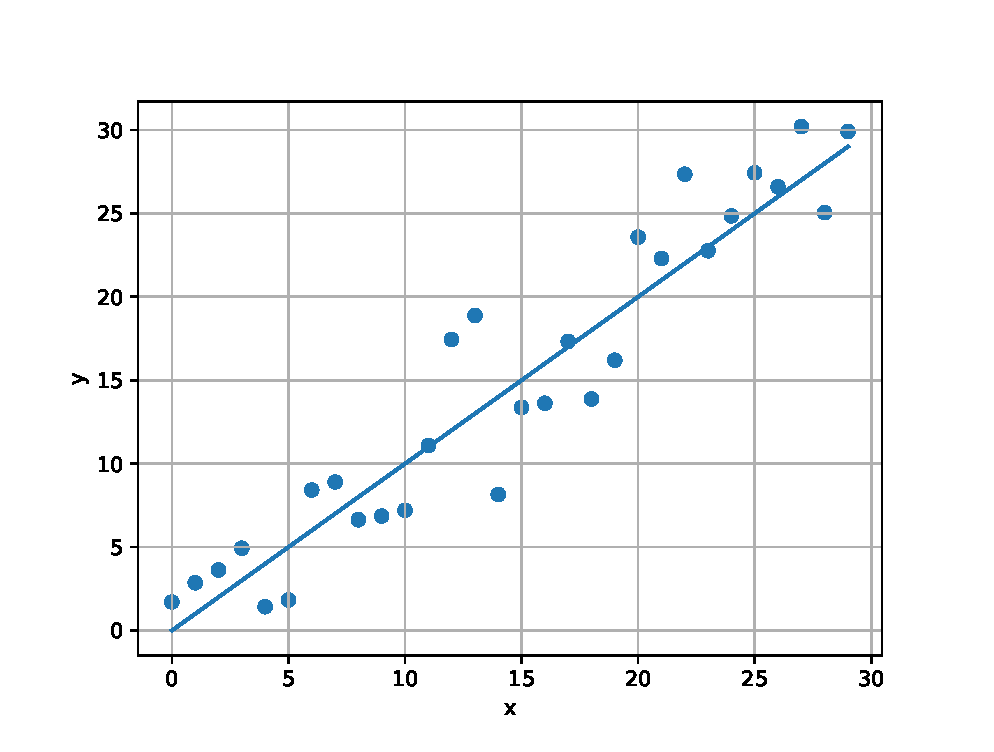
\includegraphics[width=8.0cm]{code/fig6.eps}
\vspace{-10pt}
\caption{\texttt{fig6.eps}}
\endframed
\end{center}
\end{figure}
%\begin{lstlisting}
%\end{lstlisting}
\end{cod}
\vspace{-20pt}

\subsection{3次元の曲面図}

$z=f(x,y)$の3次元の曲面図は\texttt{<axes>.plot\_surface()}で描画することができる.これを使うためには,matplotlibの\texttt{mpl\_toolkits.mplot3d}から\texttt{Axes3D}をインポートした上で,\texttt{<figure>.add\_subplots()}による\texttt{<axes>}生成時に3次元の図を書くということを明示的に指定するため\texttt{projection='3d'}を指定してあげる必要がある.また,\texttt{<axes>.plot\_surface()}で指定する配列は全て行列としての\texttt{<2d\_ndarray>}でなければならない.そのため,\texttt{np.meshgrid()}により\texttt{<2d\_ndarray>}を生成して使うのが一般的である.

\begin{gram} 
\begin{itemize}
\item \texttt{<axes>.plot\_surface(x,y,z)}: $z=f(x,y)$の型の曲面を描画する.ここで,\texttt{x,y,z}は行列としての\texttt{<2d\_ndarray>}であることが必要である.なお,このメソッドを使うためには,matplotlibの\texttt{mpl\_toolkits.mplot3d}から\texttt{Axes3D}をインポートし,\texttt{<axes>}を\texttt{<figure>.add\_subplots()}で作成するときに\texttt{projection='3d'}を指定する必要がある.
\item \texttt{<axes>.set\_zlabel(<str>)}: $z$軸のラベルを設定する.
\item \texttt{<axes>.set\_title(<str>)}: 描画した\texttt{<axes>}にタイトルをつける.
\item latex記法: matplotlibにおいて\texttt{<str>}にlatexの数式を使いたい場合,\texttt{r<str>}と書く.
\end{itemize}
\end{gram}

\begin{cod}[\texttt{fig4.py}] \\
$f(x,y)=x^2-y^2~(-5\leq x\leq 5,-5\leq y\leq 5)$のグラフを描画した例.Pythonの関数をシンプルに書いているが,\texttt{<ndarray>}の四則演算は各成分ごとの計算となることを利用して,\texttt{<2d\_ndarray>}の全成分に対して$f$の値をサクッと計算させて\texttt{<2d\_ndarray>}のまま保持するようにしている.
\lstinputlisting[backgroundcolor={\color[gray]{.95}}]{code/fig4.py}
\vspace{-19pt}
\begin{figure}[H]
\begin{center}
\framed
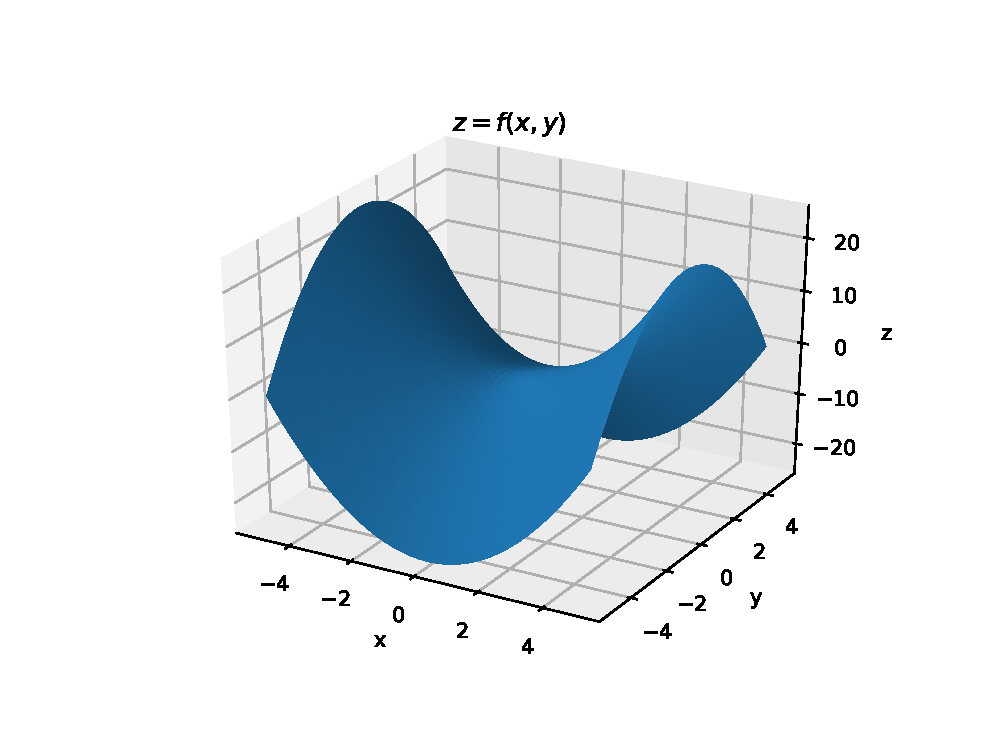
\includegraphics[width=12.0cm]{code/fig4.eps}
\vspace{-10pt}
\caption{\texttt{fig4.eps}}
\endframed
\end{center}
\end{figure}
%\begin{lstlisting}
%\end{lstlisting}
\end{cod}
\vspace{-20pt}

\subsection{2次元の等高線図}

$z=f(x,y)$の2次元の等高線図は\texttt{<axes>.contour()}で描画する.これも配列には行列としての\texttt{<2d\_ndarray>}を指定しなければならないので注意する.

\begin{gram} 
\begin{itemize}
\item \texttt{<axes>.contour(x,y,z,levels=<1d\_ndarray>)}: $z=f(x,y)$の型の等高線図を描画する.ここで,\texttt{x,y,z}は行列としての\texttt{<2d\_ndarray>}であることが必要である.等高線は,\texttt{levels=<1d\_ndarray>}を指定しない場合は$z$の値について等間隔に描画されるが,例えば$z$の値が指数的に増加する場合などは少しの$x,y$の変動で大きく$z$が動いてしまい等高線同士が詰まってしまうので,\texttt{levels=<1d\_ndarray>}に直接$z$の値を指定して,等高線を直接定めることもできる.
\item \texttt{plt.figure(figsize=(a,b))}: \texttt{figsize}は\texttt{<figure>}領域のサイズ(縦\texttt{a}インチ,横\texttt{b}インチ)を指定する.\texttt{figsize}を省略した場合は\texttt{(8,6)},すなわち横8インチ,縦6インチの指定となる.\texttt{subplot}をたくさん横につなげる場合でも\texttt{figsize}は変わらないので,つぶれたりゆがんだりする.ので,複数の図を描くときは\texttt{figsize}を検討する必要がある.
\end{itemize}
\end{gram}

\begin{cod}[\texttt{fig5.py}] \\
$f(x,y)=\frac{e^x+e^{-x}+e^y+e^{-y}}{4}~(-5\leq x\leq 5,-5\leq y\leq 5)$について曲面図と等高線図を描画した例.指数関数なので,等高線を$f$の値で等間隔でとっても$x,y$で見れば等間隔ではない.ので,右側の図では等高線の間隔を,対数をとったら等間隔になるように指定している.
\lstinputlisting[backgroundcolor={\color[gray]{.95}}]{code/fig5.py}
\vspace{-19pt}
\begin{figure}[H]
\begin{center}
\framed
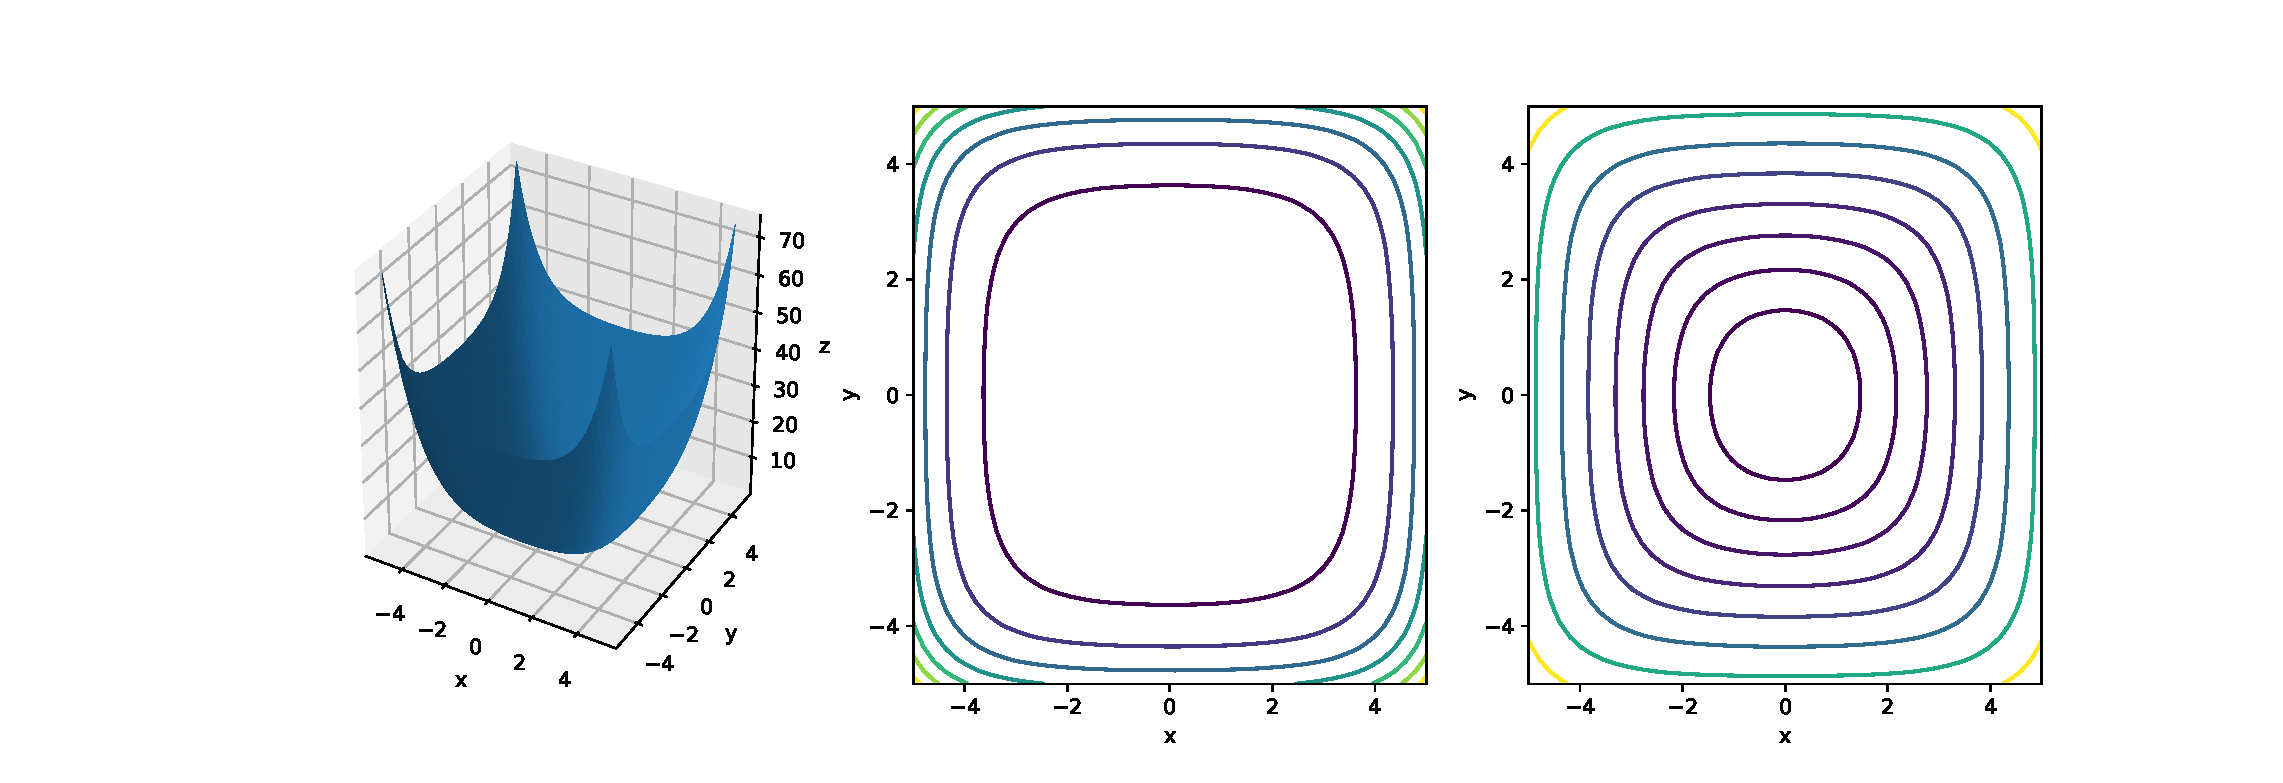
\includegraphics[width=15.0cm]{code/fig5.eps}
\vspace{-10pt}
\caption{\texttt{fig5.eps}}
\endframed
\end{center}
\end{figure}
%\begin{lstlisting}
%\end{lstlisting}
\end{cod}
\vspace{-20pt}

\subsection{\texttt{<axes>}間での$y$軸の共有}

matplotlibは,データに応じて軸の目盛りは自動調整されるが,そのせいで,グラフの見た目(傾き等)がどれも同じように調整されてしまい,グラフを比較するときに大きな誤認をしてしまう可能性がある.\texttt{<figure>.subplot()}で\texttt{<axes>}間の$y$軸を同じくする場合,\texttt{<axes>}を生成するときのオプションに\texttt{sharey=<axes>}を指定する.

\begin{gram} 
\begin{itemize}
\item \texttt{<figure>.add\_subplot(a,b,c, sharey=<axes2>)}: \texttt{<figure>}を\texttt{a}行\texttt{b}列に分割した上で,\texttt{c}番目の部分に,$y$軸を\texttt{<axes2>}と共有した空の\texttt{<axes>}を作成する.
\end{itemize}
\end{gram}
\begin{cod}[\texttt{fig8.py}] \\
\lstinputlisting[backgroundcolor={\color[gray]{.95}}]{code/fig8.py}
\vspace{-19pt}
\begin{figure}[H]
\begin{center}
\framed
\includegraphics[width=15.0cm]{code/fig8-1.eps}
\vspace{-10pt}
\caption{\texttt{fig8-1.eps}}
\includegraphics[width=15.0cm]{code/fig8-2.eps}
\vspace{-10pt}
\caption{\texttt{fig8-2.eps}}
\endframed
\end{center}
\end{figure}
%\begin{lstlisting}
%\end{lstlisting}
\end{cod}
\vspace{-20pt}
